This section contains the main problem for this project and the generic description of the required solution.

\subsection{Analysis Summary}
The analysis was based on the initial problem: \textit{How can the current \citybike system be improved, in order to make it more usable?}.
From the analysis, it was found that the current \citybike has several problems, limiting the overall usability (as described in \Cref{aalborg_bycyklen:challenges}).

The problems identified were:
\begin{enumerate}
\item Bikes left outside stations \label{pr_stations}
\item Too few stations \label{pr_few}
\item Making short stops \label{pr_stops}
\item No bikes at station \label{pr_nobikes}
\item No way of knowing when a bike will arrive \label{pr_arrive}
\item Broken bikes \label{pr_broken}
\end{enumerate}

Additionally, certain limitations and requests were made by Aalborg Kommune, collected through the interview:

\begin{enumerate}
\item No renting/booking system
\item No specific target user group
\item Interested in statistics about usage \label{pr_stats}
\item Short period usage
\end{enumerate}

\subsection{Scope}
Due to the limited time and project members restrictions will be set, to remove focus from certain problems.

\paragraph{\ref{pr_stops}: Making short stops} The problem about making short stops is not solved directly, as the only solution we see can directly address the problem, is the use of a locking mechanism.
This would conflict with the limitations set by Aalborg Kommune.

\paragraph{Statistics about usage} The request from Aalborg Kommune to provide statistics, is deemed too far from the initial problem, as we won't be able to get any significant data without testing it on the actual bikes.

\subsection{Solution} \label{prob_statement:solution}
We have chosen the solution with the same bikes as the current system, with the addition of a GPS receiver on each individual bike, and completely removing the stations and bike locks.
This is due to the restrictions set by Aalborg Kommune, requesting a simple system, in order to accommodate the unspecified target user group.


\paragraph{GPS receivers and Hotspots}\label{gpsreceiver}
The greatest changes to the current system is the addition of the GPS receivers and the introduction of hotspots.
As we do not have access to real GPS receivers, we will base the rest of the report on the following assumptions about the GPS receivers on the bikes:
Each bike is equipped with a GPS receiver which uses GPS satellites to calculate its location. The GPS receiver is presumed to send the location of the receiver, an accuracy stated in meters\footnote{the definition of accuracy is based on the output from \citet{followmee}} and a time stamp indicating the time of the reading.
This collection of data will be referred to as a \emph{GPS location}	
The GPS receiver will send a GpS location to our system at a fixed interval, but it is not guaranteed that the interval is exact.

Hotspots will serve as informal stations; areas of the map where bikes are often parked.

By combining these two things, we want to improve on the problems with the current system.

\subparagraph{\ref{pr_stations}: Bikes left outside stations} The problem is handled by the GPS receivers, as bikes and their location now can be found, no matter if it is at a hotspot or not.

\subparagraph{\ref{pr_few}: Too few stations} By generating hotspots this problem is handled.
Whenever an area is a popular place to be going from/to, a hotspot should emerge and reflect this.

\subparagraph{\ref{pr_stops}: Making short stops} This problem is improved upon but not solved.
If a user stops in a hotspot he can use the system to estimate how long he will have to wait before a new bike arrives at that particular hotspot.
From this information he can decide whether to leave the bike or not (or possibly how long he should spend in a shop etc.).
This is an improvement over the current system that provides no such information, however it does not solve the problem entirely.

\subparagraph{\ref{pr_nobikes}: No bikes at station} Locating the exact location of an available bike, or looking up nearby hotspots, should handle this problem.

\subparagraph{\ref{pr_arrive}: No way of knowing when a bike will arrive} This problem is addressed by modeling bike behavior and predicting when a bike will be available at certain hotspot(s).

\subparagraph{\ref{pr_broken}: Broken bikes} We will not directly handle this problem, but it is possible to infer from looking at bike locations and detecting when a bike has been immobile for a very long time, which could indicate that it either is too far away for anyone to pick it up, or broken.
\alexander{Se om ovenstående paragraffer nu er acceptable efter ikke længere at titlen er en del af sætningen.}
\paragraph{Software}
A software solution is to be developed, consisting of 3 main software components, and a shared database.
The structure of the solution can be seen in \Cref{fig:solution_structure}.

\begin{figure}[h]
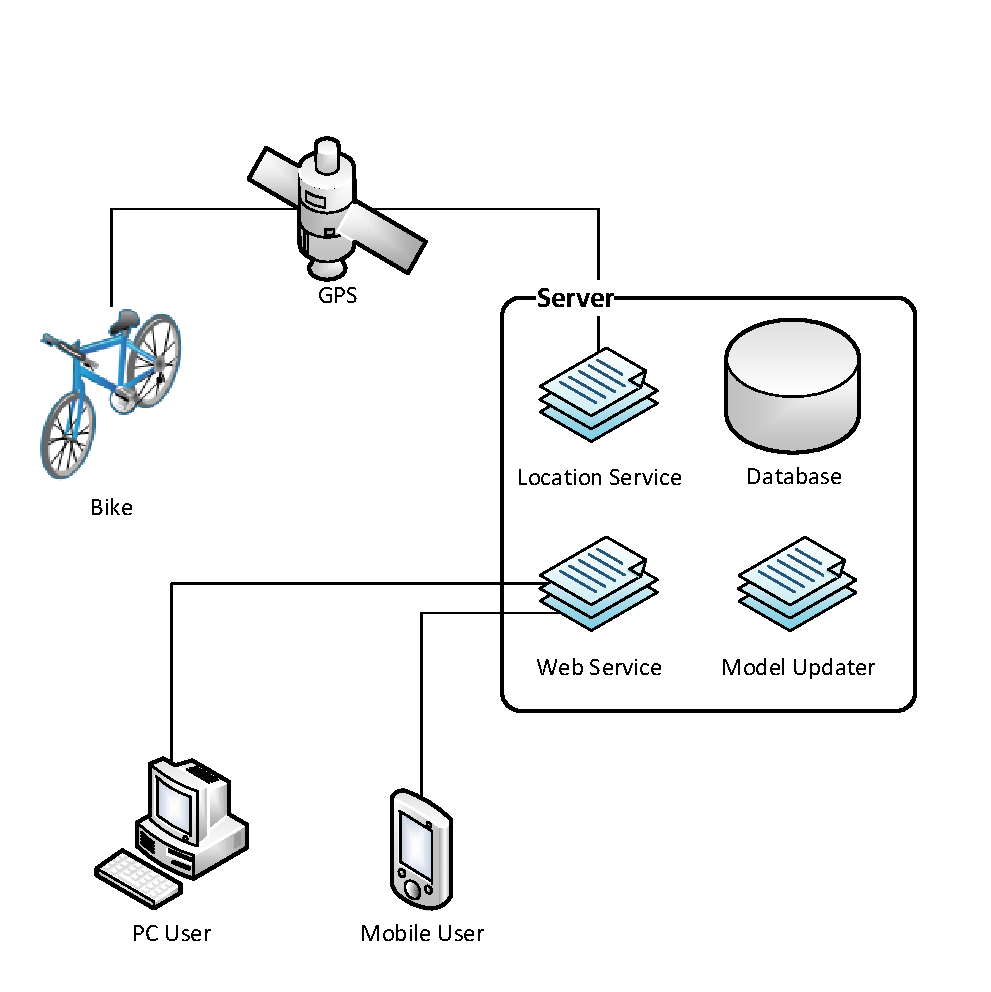
\includegraphics[width=\textwidth, trim={0cm 1cm 2cm 1.5cm}]{our_solution.pdf}
\caption{The overall structure of our solution}
\label{fig:solution_structure}
\end{figure}

The \textit{Location Service} continuously updates the locations of the bikes.
The \textit{Model Updater} uses the stored location data to generate a model used for predictions.
The \textit{Web Service} makes an API available, in order to make platform implementations to make the data available as specified in the requirements.
A web service was chosen as to make the system as available as possible, due to the unspecific target user group.

\subsection{New problems} \label{new_problems}
In order to develop this system, with the addition of GPS receivers and hotspots, new problems emerge.
The following chapters will focus on these problems:

\begin{itemize}
\item Defining and identifying hotspots
\item Modeling the usage and using the model for predictions
\item Making the data available through a web service
\end{itemize}
